% History
% 12/06/2024  (岸)	修論下書き用texファイル作成
% 12/12/2024  (岸)	フォントサイズを11pt, 行間を1.5に設定
% コンパイルの仕方
% 		uplatex chapter1_v1.tex
% 		pbibtex chapter1_v1
% 		uplatex chapter1_v1.tex
% 		uplatex chapter1_v1.tex
% 		dvipdfmx chapter1_v1.dvi

% フォントサイズを11ptに設定
\documentclass[a4paper,11pt,nomag]{jsreport}

\usepackage[dvipdfm,truedimen]{geometry}
\geometry{top=22mm,bottom=22mm,left=22mm,right=22mm}
%% jsclasses系で文字サイズ11pt や 12pt をクラスオプションに指定すると,
%% 長さが拡大されるため,nomagオプションを併用している.
%% https://oku.edu.mie-u.ac.jp/~okumura/jsclasses/ のFAQをよく読むこと.

%\usepackage{layout}
%\usepackage[utf8]{inputenc} %不要かも
\usepackage[T1]{fontenc} %utf8フォントエンコーディング指定
\usepackage{lmodern} % 11pt, nomag を使っているので
% CloudLaTeX の場合は下の1行を有効にすること
% \AtBeginDvi{\special{pdf:mapfile ptex-ipaex.map}}
\usepackage{array}
\newcommand{\bhline}[1]{\noalign{\hrule height #1}}  
\newcommand{\bvline}[1]{\vrule width #1}
\renewcommand{\baselinestretch}{1.5} % 教授が赤修正を入れやすいように行間を1.5に設定
\usepackage[subrefformat=parens]{subcaption}
\usepackage[dvipdfmx]{graphicx} % dvipdfmx を前提としている
\usepackage[dvipdfmx]{color}
\usepackage{caption}
\usepackage{subcaption}
\usepackage{bbm}
\usepackage{multirow}
\usepackage{arydshln}
\usepackage{here} % 図表の位置決め用
\usepackage{amsmath,amssymb}% 数式用
\usepackage{url}      % URL等記載用.\verbより便利
\usepackage{enumerate}
\usepackage{midpage}

% サブキャプションのフォーマットを調整
\renewcommand\thesubfigure{(\alph{subfigure})}
\captionsetup[subfigure]{labelformat=simple, labelsep=space}

\begin{document}
\setcounter{chapter}{2}

\chapter*{深層学習を用いた動物分類に関する既存研究}

\section{赤外線画像に対する既存研究}

気候変動や人口増加が生態系に与える影響を把握することは、野生動物と人間の共存において重要な課題である。
この課題を解決するため、生態系モニタリングの重要性が世界的に高まっている。
具体的には、監視カメラなどを用いることにより、特定地域の動物種の個体数の推定だけではなく、その環境においての各種の行動や生態について観察や研究が行われている。
特に,野生鳥獣の監視ツールとして,人間が直接関与せず,また,生態系への影響が極力少ない遠隔での自動撮影を行うカメラトラップが広く使用されている.
カメラトラップは,モーションセンサや赤外線センサによって自動での撮影を可能にしているため,人間の労力削減と24時間のモニタリングが可能である.
また,野生鳥獣が現れそうな場所の樹木や地面にカメラを固定するだけの単純な設置方法であることも利点である.
カメラトラップを使用した撮影では,数年間にわたった撮影期間や,多くの撮影箇所の設定などによって,膨大な画像枚数を取得していることも少なくない.
しかしながら,記録された画像・映像中から鳥獣の有無や種の推定を人手で行うことは多大なコストを要する.
加えて,種の分類には専門的な知識が必要であることも作業員確保のコスト面での課題である.
したがって,これらの課題を解決するため,カメラトラップによって撮影された画像・動画中から自動で動物を検出・識別する手法の実現が望まれている.

近年では,画像処理技術と機械学習を用いた野生鳥獣の自動識別手法が研究されている.
2012年の画像処理タスクに関連する深層学習技術の登場以降,画像処理分野の様々な分野においてCNNに基づく手法が盛んに研究されている.
また,その多くの分野においてCNNは高い性能を実現しており,カメラトラップによる動物識別に関する研究においてもCNNを用いた手法がいくつか提案されている.
Tanら \cite{tan2022}は,2014年から2020年にかけて撮影された約25,000 枚の自作データセットを用いて,YOLOv5,FCOS(Fully Convolutional One-Stage ObjectDetection),Cascade R-CNNの3つの検出ネットワークでの比較検証をおよび映像に適用した動物認識の性能を評価している.
Tabakら \cite{tabak2019}は,全米5か所で撮影された約300万枚のカメラトラップ画像を用いて,独自のCNNにより動物の画像分類を行っている.

しかしながら,上記のような既存研究の分類モデルを学習するために用いられた大規模なデータセットは,多くの撮影場所や長期間に渡った撮影によって蓄積された画像で構成されている.
したがって,これらの既存研究は,個人的な利用での撮影や狭い範囲の地域での撮影など,多くの画像を集められるとは限らない状況を考慮していないため実用的では無い.
また,夜間に行動する動物の撮影には赤外線を用いることが有効である.
しかし,図2.1.1 で示すように赤外線で撮影された画像は色情報を含まないなど,可視光で撮影された画像とは映り方が異なる.
したがって,真に実用的な夜間の動物モニタリングの実現に向けて,少数の赤外線で撮影された画像のみでも学習可能な深層学習モデルについての検討が急務である.

このような既存研究の課題解決に向けた研究として,少数の赤外線画像を用いた動物分類が挙げられる.
Kishiら[1]は,米国南西部の140 か所で撮影された画像3000 枚を用いて,CNN による少数の赤外線画像を用いた動物分類を行っている.
また,少数のデータを用いて深層学習モデルを効果的に学習させることを目的とするFew Shot Learning (FSL) の分野において有効な手法である転移学習とデータ拡張の赤外線画像に対する有効性を検証した.
転移学習は,事前に大量のデータを用いて学習したモデルを新しいタスクに用いる手法であり,本研究では,画像認識タスクに一般的に用いられるデータセットであるImageNet とImageNet を擬似赤外線化した画像,さらに数式から生成されたフラクタル画像による転移学習の有効性をそれぞれ検証した.
一方,データ拡張については,一般的な画像変換によるデータ拡張と画像の一部をマスクし隠すことでモデルの汎化性能を向上させるRandom Erasing,画像処理後の画像を組み合わせることで新しい画像を生成しモデルの頑健性を向上させるAugmixなどの有効性を比較検証した.
結果として,転移学習では疑似赤外線画像,フラクタル画像,ImageNet の順に効果があることが示された.
また,データ拡張においては,最新の手法であるAugMix が特に有効であると結論づけられている.
しかし,Kishi らの研究の課題として,転移学習では通常大量のデータでモデルを学習する手法であるが,本研究では1 クラスあたり100 枚という限られたデータのみを使用している.
そのため,厳密には転移学習ではなく,別ドメイン画像を用いたファインチューニングによる,少数の赤外線画像分類への有効性の検証を行った研究だと解釈できる.
よって,転移学習を赤外線画像タスクに用いた際の有効性は検証できていない.
また,データが少ない状況を想定し,学習に使用する画像は600 枚としているが,実運用を想定した場合では600 枚程度の収集すら困難な場合も考えられる.
さらに,モデルの評価実験におけるテスト用データセットには学習時と同じ動物のクラスが使用されていることから,運用する地域ごとに600 枚程度の学習データを集めることが前提の研究となっている.
つまり,一度学習したモデルを別地域にて即時に適用することが困難だと考えられる.
そして,赤外線画像に対する事前学習やデータ拡張の評価を行っているものの,一般的なカラー画像との比較が行われていない.
したがって,各手法が赤外線画像のみに対して効果的であるか,それとも一般的な画像分類においての精度向上に寄与しているのかを判断することができない.

特に重要な課題として,モデルの学習に使用されるデータに含まれる動物種が少ない場合,実用時には学習データに含まれなかった動物が出現することが挙げられる.
一般的な分類モデルは,そういった未見の動物を正しく識別できず,学習済みのクラスに強制的に分類してしまう.
図2.1.2 は,一般的な分類モデルが未見動物を識別できない例を示している.
図2.1.2 で示される通り,一般的な分類モデルは分類したい画像を,画像から抽出した特徴量が類似している既存クラスに分類するため,未見データであっても等しく既存クラスに分類されてしまう.
そのため,もし学習時データに含まれない危険な動物が実用時に現れた場合,モデルは判別することができず,重大な事故を引き起こす可能性がある.

以上より,未見の動物を識別できるモデルの開発は急務である.
なお,未見の識別を行う能力をモデルに付与する問題設定をオープンセット認識(Open Set Recognition, OSR) と呼ぶ.

% \begin{figure}[tbp]
%   \centering
%   \begin{subfigure}[b]{0.45\linewidth}
%     \centering
%     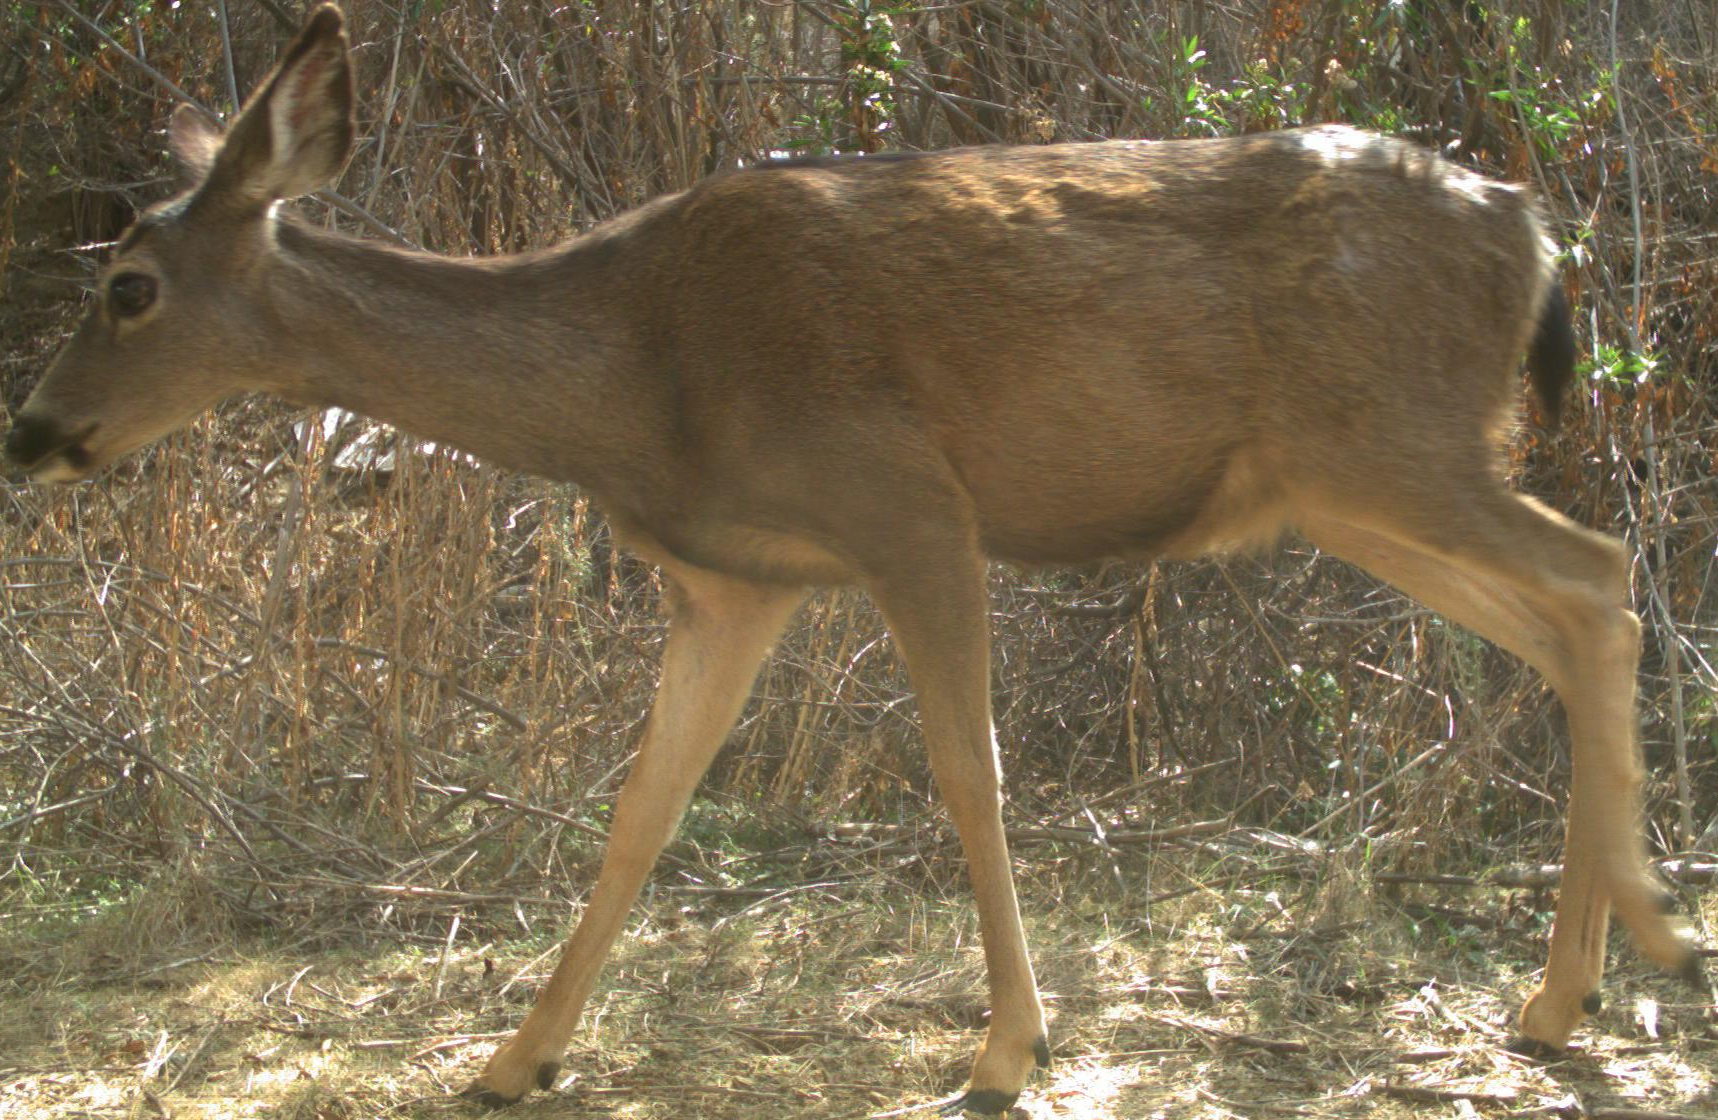
\includegraphics[height=0.7\linewidth, keepaspectratio]{cct_color_deer.png}
%     \caption{可視光画像}
%     \label{fig:color_deer}
%   \end{subfigure}
%   \hfill
%   \begin{subfigure}[b]{0.45\linewidth}
%     \centering
%     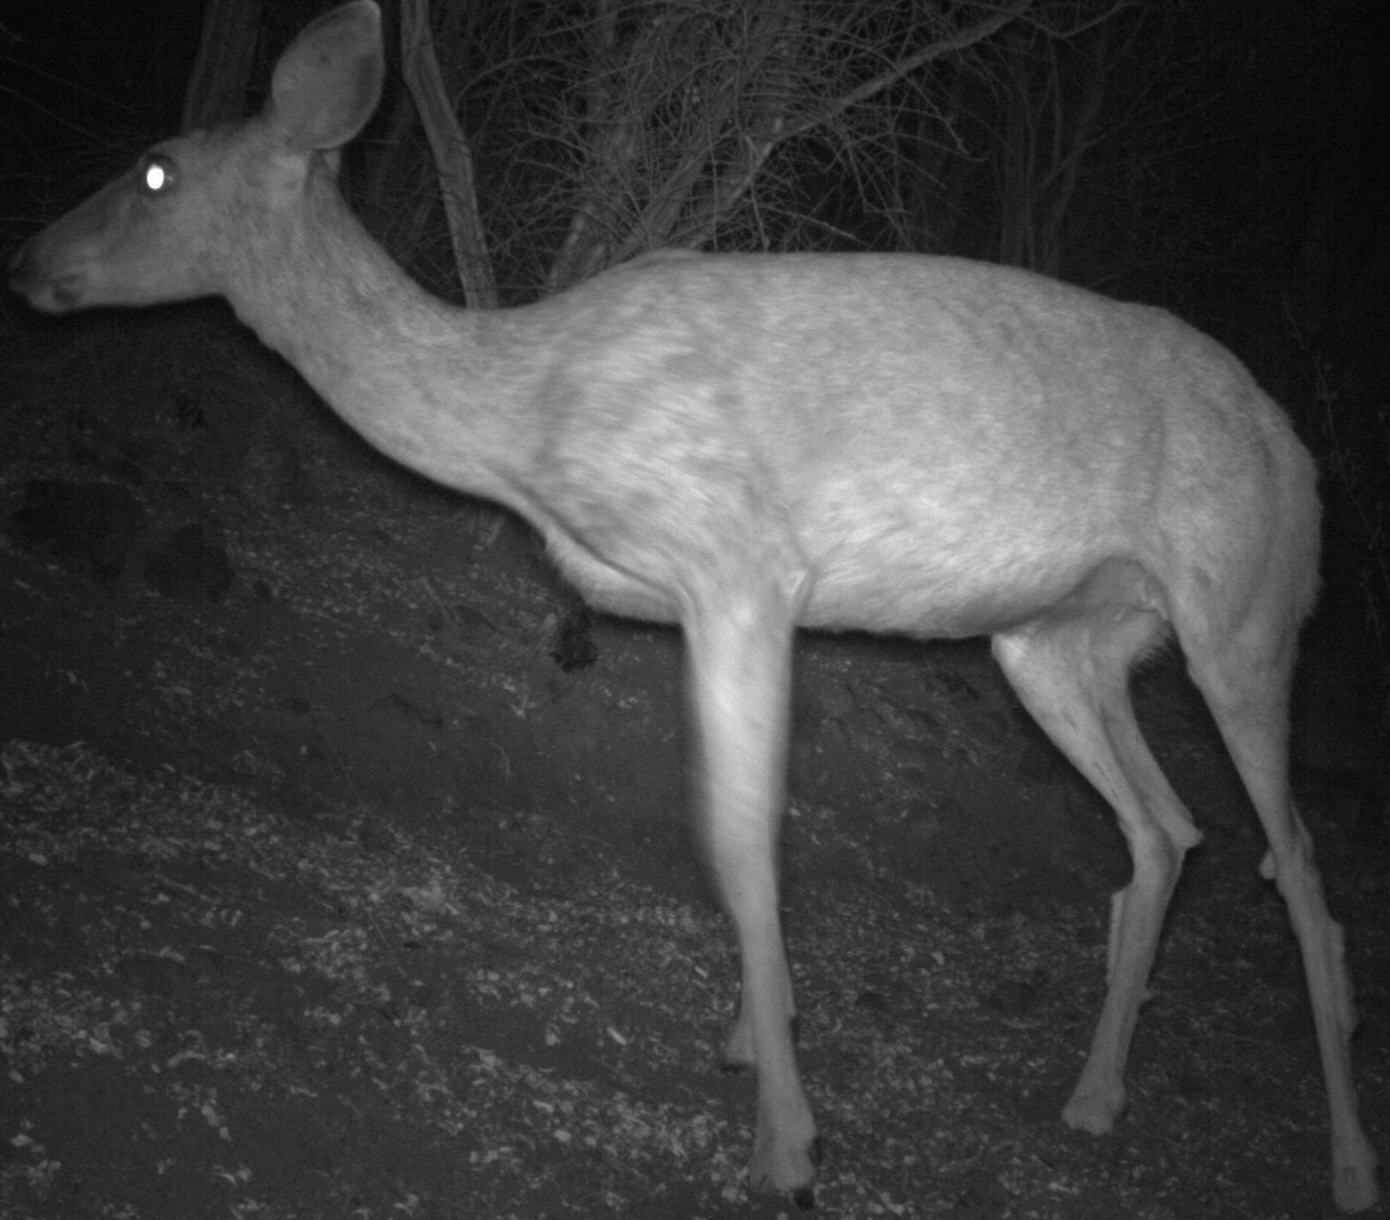
\includegraphics[height=0.7\linewidth, keepaspectratio]{cct_infrared_deer.png}
%     \caption{赤外線画像}
%     \label{fig:infrared_deer}
%   \end{subfigure}
%   \caption{撮影方法の違いによる物体の写り方}
%   \label{fig:camera}
% \end{figure}

このような課題を解決するため,少数の赤外線画像を用いた動物分類の研究が行われている \cite{kishimoto2023}.
しかし,既存研究では,評価時に分類対象となる動物種は全て学習済みであると仮定しているが,実運用において,深層学習モデルを特定の地域に適用する際,モデルが対象地域に生息する全ての動物種を学習しているとは限らない.
このような状況において,未学習の動物種は学習済みの動物種に強制的に誤分類され,モデルの性能は著しく低下することが知られている.
この問題はオープンセット問題 (Open-Set Problem) と呼ばれ,この問題に対処するため,学習済みクラスの分類を行いつつ,未学習クラスを検出するオープンセット認識 (Open-Set Recognition,OSR) 手法が提案されている \cite{sun2020, sagar2022}.

さらに近年では,少数データでもオープンセット認識を可能にする Few-Shot Open-Set Recognition (FSOSR) \cite{peeler} が注目を集めている.
代表的なFSOSR手法として,少数データ学習 (Few-Shot Learning,FSL) 分野で有効な手法とされているメタ学習をOSRに拡張することによりFSLとOSRを同時に実現したPEELER \cite{peeler}や,変換の一貫性に基づき未学習クラスを検出することによって,擬似的な未学習クラスサンプルを必要としないSnaTCHer \cite{snatcher}が挙げられる.

しかし,これらの手法は可視光画像を対象としており,赤外線画像に対して性能評価がなされていない.
また,FSOSRでは未学習クラスを単一種として扱っているが,未学習クラスのアノテーションや追加学習を考慮すると,実用的には未学習クラスも複数種に分類できることが望ましい.

本論文では,夜間の野生動物モニタリングの実現を目的とした,より実用的な問題設定である「Infrared Few-shot Open-set Recognition (IFOR)」を提案する.
IFORでは少量の赤外線画像データのみを用いて,特定地域に生息するモデルに学習済みの動物種を正確に分類し,かつ,未学習の動物種の検出を可能にすることを目指す.

加えて,IFORではドメインシフトに対する頑健性の評価も行う.
ドメインシフトとは,学習データと評価データが異なる地域で収集された場合に生じる課題であり,背景や撮影環境の違い,同じ動物種の地域差による外見の違いによってモデルの性能が低下する現象を指す.
ドメインシフトを考慮することにより,地理的条件に依存せず,様々な場所に適用可能な汎用性の高いシステムの実現が期待される.

IFORの実現に向けて,赤外線画像に有効な既存手法の特定に加え,既存のFSOSR手法の1つであるメタ学習フレームワークがIFORに対して効果的であるか検証を行う.
まず,赤外線画像に有効な特徴抽出器を特定するため,テクスチャ特徴に焦点を当てているCNNや,形状特徴 \cite{feature}を重視することで知られている Vision Transformer (ViT) \cite{vit}などの代表的な特徴抽出器の有効性を赤外線画像に対して評価する.
次に,IFORフレームワーク内のFSLタスクに有効なアプローチの1つである転移学習について検証する.
転移学習では,事前学習のタスクと本番環境でのタスクの類似度が重要だと考えられている.
そこで,一般的なImageNetデータセットを用いた事前学習と並行して,事前学習に色情報を持たないフラクタル画像を用いるFormula-Driven Supervised Learning (FDSL) \cite{fdsl}の有効性を探る.
最後に,赤外線画像を分類する際,小規模データセットから汎用的な特徴抽出を行うための学習戦略であるメタ学習のIFORにおける有効性を,ドメインシフトの条件下で評価する.
特に,IFORにおいては学習済みクラスの正確な画像分類と未学習クラスの検出が不可欠であるため,メタ学習による有効性を従来の学習方法であるミニバッチ学習と比較する.

さらに,IFORを発展させ,未学習クラスに対する多クラス分類の精度向上にも取り組む.
% さらに,IFORを発展させ,未学習の動物種を複数クラスに分類する課題にも取り組む.
特徴空間上で各クラス分布がコンパクトに表現されることによって多クラス分類が容易になると仮定し,クラスタリンに基づく損失関数を用いてクラス内分散の最小化・クラス間分散の最大化を図る.
クラス内分散の最小化では,異常検知タスクで用いられているk-means損失 \cite{k-means} を導入する.
クラス間分散の最大化では,k-meansクラスタリングによって得られる各クラスタ中心を利用した損失関数,Between-Class損失 (BC損失) を提案し,性能評価を行う.

以下,第2章では深層学習を用いた動物分類に関する既存研究について述べる.
第3章では夜間の野生動物モニタリングの実現に向けてより実用的な問題設定を提案し,様々な手法の有用性について述べる.
第4章では評価実験を行い,その結果及び考察を多面的な方向性から述べる.
最後に第5章では結論を述べる.

\subsection{Few-Shot Open-Set Recognitionに関する既存研究}



% ここから参考文献bibtexの設定
\bibliographystyle{../kishiIEEEtr}
\bibliography{../references}

\end{document}